%\documentclass{article}
\documentclass{www2010-submission}
\usepackage{times}
%\usepackage{uist}
\usepackage{url}
\usepackage{graphics}
\usepackage{color}
%
%\newcommand{\want}[1]{{[\color{blue} WANT: #1]}}
%\newcommand{\todo}[1]{{[\color{blue} TODO: #1]}}
%\newcommand{\idea}[1]{{[\color{blue} IDEA: #1]}}
%\newcommand{\node}[1]{{[\color{blue} NOTE: #1]}}

\newcommand{\want}[1]{}
\newcommand{\todo}[1]{}
\newcommand{\idea}[1]{}
\newcommand{\node}[1]{}


\begin{document}

\toappear

\bibliographystyle{plain}

\title{Highlighting Disputed Information on the Web}

%%
%% Note on formatting authors at different institutions, as shown below:
%% Change width arg (currently 7cm) to parbox commands as needed to
%% accommodate widest lines, taking care not to overflow the 17.8cm line width.
%% Add or delete parboxes for additional authors at different institutions. 
%% If additional authors won't fit in one row, you can add a "\\"  at the
%% end of a parbox's closing "}" to have the next parbox start a new row.
%% Be sure NOT to put any blank lines between parbox commands!
%%

\numberofauthors{5}

\author{
	Author list to be determined
}

%\author{
%\alignauthor Rob Ennals\\
%       \affaddr{Intel Labs Berkeley}\\
%       \affaddr{2150 Shattuck Ave}\\
%       \affaddr{Berkeley, CA, USA}\\
%       \email{robert.ennals@intel.com}
%\alignauthor Beth Trushkowsky\\
%       \affaddr{Computer Science Division}\\
%       \affaddr{University of California at Berkeley}\\
%       \affaddr{Berkeley, CA, USA}\\
%       \email{trush@berkeley.edu}
%\alignauthor John Mark Agosta\\
%       \affaddr{Intel Labs Santa Clara}\\
%       \affaddr{2200 Mission College Blvd}\\
%       \affaddr{Santa Clara, CA, USA}\\
%       \email{john.m.agosta@intel.com}
%}
%
%\additionalauthors{Additional authors: Tad Hirsch (Intel Research PaPR, email: {\texttt{tad.hirsch@intel.com}}) and Tye Rattenbury (Intel Research PaPR), email: {\texttt{tye.rattenbury@intel.com}})}


\maketitle

%RULE: Don't cite media reports unless I have to - some reviewers don't like it


\abstract

We describe Dispute Finder, a browser extension that alerts a user when information they read online is disputed by a source that they might trust. Dispute Finder examines the text on the page that the user is browsing and highlights any phrases that appear to entail claims in its database of known disputed claims. If a user clicks on a highlighted phrase then Dispute Finder will show the user a summary of articles that support other points of view.

Dispute Finder builds it's database of disputed claims by crawling web sites that already maintain lists of disputed claims, and by allowing users to enter claims that they believe are disputed. Dispute Finder identifies instances of disputed claims by running a simple textual entailment algorithm inside the browser extension, referring to a cached local copy of a subset of our claim database.

Performing these tasks well is a hard problem, and we do not yet claim to have an implementation that is good enough to be compelling for most users. We do however believe that Dispute Finder attacks an interesting problem that, if addressed well, could significantly improve the utility of the web.

\category{H.4.m}{Information Systems}{Miscellaneous}
\category{H.4.2}{Information Systems}{Decision Support}
\category{H.5.2}{User Interfaces}{Graphical User Interfaces}

\terms{Design, Human Factors}

\keywords{Sensemaking, Annotation, Argumentation, Web, CSCW}


\tolerance=400 
  % makes some lines with lots of white space, but 	
  % tends to prevent words from sticking out in the margin

\section{INTRODUCTION}

\todo{update screenshots}
\todo{should this be spun as about news, or information in general}
\todo{need to talk more about what we know about people}
 
% The last few years have seen the rapid decline of printed newspapers and rapid rise of the web as a source of news~\cite{pew-news?}.

The web contains a huge amount of information, but some of this information is factually incorrect~\cite{Neumann2003,Resnik1998,Zhou2004} and some sites present only one side of a contentious issue~\cite{Herman2002}. If a user is to gain a broad understanding of a topic then they will need to either spend time looking for alternative points of view, or restrict themselves to sources that they believe they can trust to provide accurate and balanced information.


\begin{figure}[tb]
	\begin{center}
	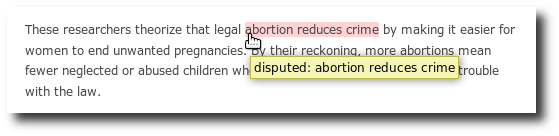
\includegraphics[width=8cm]{pictures/highlight_abortion.png}
	\caption{A highlighted snippet that makes a disputed claim}
	\label{highlight}
	\end{center}
\end{figure}

\begin{figure}[tb]
	\begin{center}
	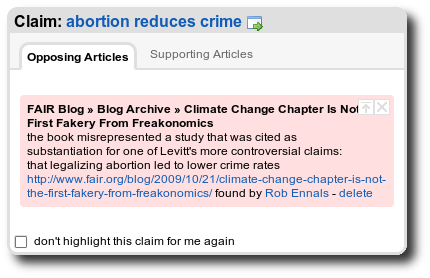
\includegraphics[width=6cm]{pictures/popup_abortion_shadow.png}
	\caption{Popup interface with articles for and against a claim}
	\label{claimview}
	\end{center}
\end{figure}
\todo{Popup interface should contain a "don't mark this" button}

\todo{More screenshots/graphs/visual information}

In the realm of News, Pew~\cite{pew-news} report that, while internet news is rapidly gaining ground on traditional news sources, most online news sources are not considered credible. Even when users are getting news from the websites of traditional news providers, it is likely that they read news from a variety of unfamiliar news sources~\cite{pew-news}, rather than the small set of newspapers and TV stations that they might have followed in the past.

\todo{word this better}\todo{update all screenshots}

In this paper we describe Dispute Finder, a tool that alerts a user when information they read online is disputed by a source that they might trust. Our hope is that Dispute Finder will make it easier for a user to gain a broad view of a topic that they are interested in, understand why other people hold different points of view, and avoid being mislead by misinformation.

A user can install Disute Finder as an extension to the Firefox\footnote{http://www.mozilla.org/firefox} web browser. When installed Dispute Finder will highlight snippets of text that make disputed claims (Figure~\ref{highlight}). 
If a user clicks on a highlighted snippet, Dispute Finder will show articles that put forward different points of view,  each of which is from a source we believe the user is likely to trust (Figure~\ref{claimview}). 

\begin{figure}[tb]
	\begin{center}
	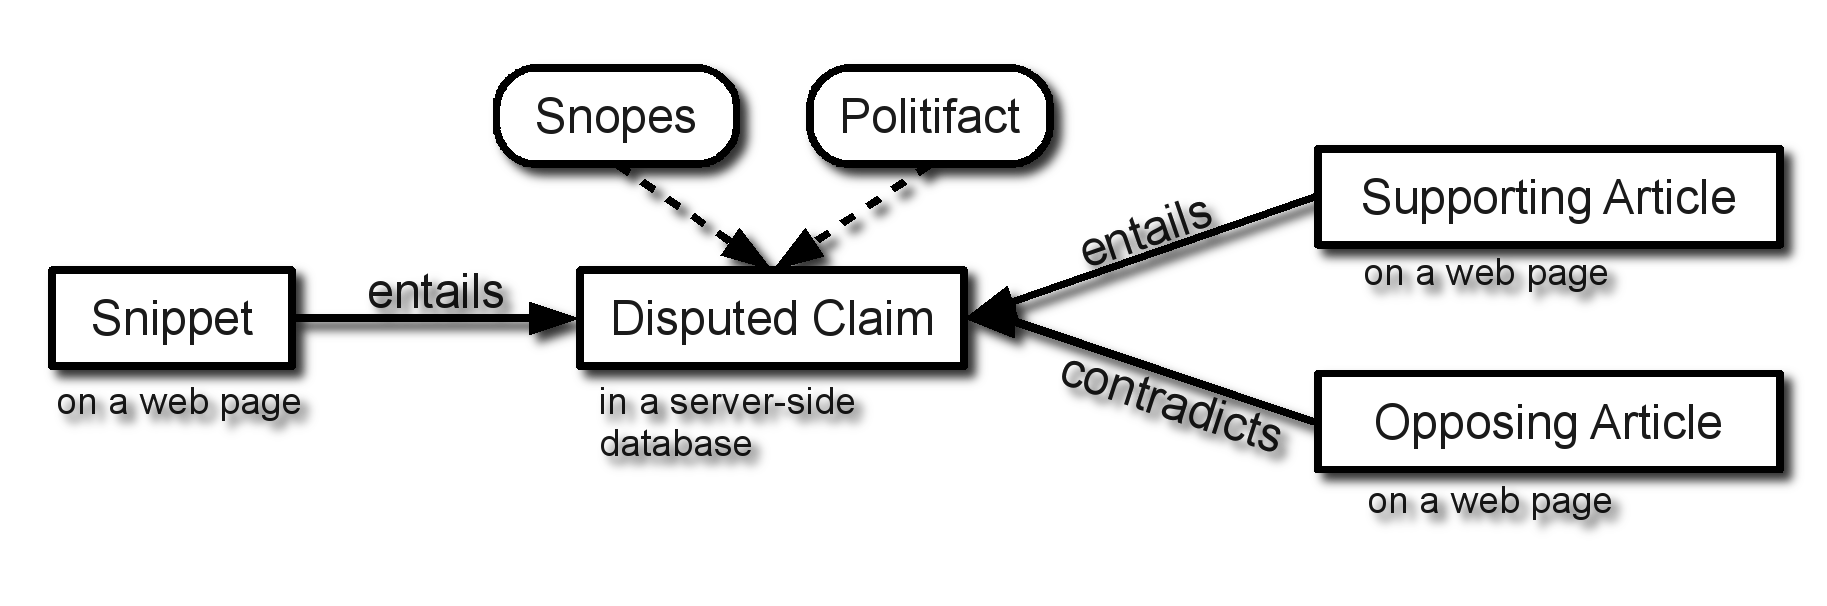
\includegraphics[width=8cm]{pictures/snippet_claim_article_fancy2.png}
	\caption{Snippets entail claims, which are entailed or contradicted by articles}
	\label{snippet_claim_article}
	\end{center}
\end{figure}

Dispute Finder consists of a database, an API, and a Firefox browser extension. The database contains a set of known disputed claims that appear on the web, articles that support or oppose each disputed claim, and hints about how to determine whether a text snippet entails a known disputed claim (Figure~\ref{snippet_clim_article}). The API allows an external client to access the information in the database and use it to tell whether particular text is likely to be making a known disputed claims. The Firefox extension uses the API to determine whether the web page a user is viewing makes disputed claims. The API could also be used by other services that present users with potentially-disputed content, such as search engines, news readers, email programs, or content management systems.

\todo{Figure that does a smaller highlight}

There are several design decisions that must be made when building a system such as this. In particular:

\begin{description}
\item[What is disputed?] To be useful, the set of known disputed claims needs to be both large (so a user is likely to see snippets highlighted reasonably often) and accurate (so users aren't distracted by things that they would not consider to be disputed). We currently use a combination of crowdsourcing from users, and mining web sites such as Snopes and Politifact that already maintain lists of disputed claims. More generally, the challenge is not to determine if a claim is disputed by {\it anyone} but to determine whether there is an alternative point of view that this particular user would take seriously.

\item[How do we find disputed snippets?] Given a particular web page, how do we determine which phrases on that page are making known disputed claims? We have experimented with several different approaches, each of which has different advantages and disadvantages. One can ask users to mark snippets individually. One can build a search tool that allows a user to find and mark similar snippets in bulk. One can provide an interface that allows a user to train a machine learning classifier to recognize snippets. One can run a textual entailment algorithm on the client that looks for phrases that look similar to a known claim. 

\item[How do we highlight snippets?] How do we tell what web page a user is reading, and augment their interface to alert them about disputed claims? Using a browser extension allows us to examine all content the user browses, but limits us to users who are prepared to install a browser extension. Using a proxy~\cite{Barrett1997} has similar adoption problems to a browser extension, and is likely to break some web sites. If external sites such as news readers and search engines use our API then they can provide information about disputed claims to users without them having to install anything, but this limits coverage to content accessed through sites that use the API.

\item[How should we explain a disputed claim?] If someone requests more information about a disputed claim by clicking on a highlighted snippet, what information should we show them that will help them decide whether to consider alternative points of view? We tried an argumentation graph and lists of articles that support or oppose the claim.
\end{description}


If users are going to adopt Dispute Finder, it is important that it provides users with a service that they feel will be of benefit to them, and has an interface that they can use. Dispute Finder is designed to cater to two personas. Each persona was created from interviews we conducted with people who we believe fit into these categories.

{\it Skeptical Readers} want to know when something they read is disputed by a source that they might trust. Their are skeptical about the accuracy of the information that they read and often check multiple sources to get different opinions on a topic. A user may behave like a skeptical reader for some topics and not others. For example a user may be skeptical when reading about topics that affect them (e.g. health, things important to their job, or things they are expected to be knowledgable about), but disengaged when reading about topics that don't affect them (e.g. entertainment) or topics for 
\todo{Use interviews to get some actual observations here. These are just fillers.}

{\it Activists} care strongly about particular issues and are prepared to spend some time helping others know that something that they disagree with is disputed. They are the same kinds of people who join protest groups, write blogs, email news stories, or argue about topics online. They are motivated by a desire to influence others and to gain status by being seen to do so. A user is likely to be an activist on some issues, but not for others. An activist will often also be a skeptical reader.

Many users fall into neither of these two personas. If a user does not regularly read information online that they feel they need to need to understand well, or restricts their reading to sources that they believe they can trust, then Dispute Finder is unlikely to be useful for them.

We used several different methods to gain input from users. We performed three rounds of users studies, circulated a survey within a target group, and conducted a series of interviews. We discuss the conclusions of these studies throught the paper, and in a section at the end. These studies were intended to inform the design of Dispute Finder, rather than to validate it. The only way to conclusively demonstrate that Dispute Finder is useful would be for it to be adopted by many active users -- something that the current implementation is not mature enough to support.

\todo{Improve the paraphraser UI so it shows users what pages are making the claim}
\todo{Improve the ``see examples on the web'' UI to it shows the pages that were found with the activists training work}
\todo{Provide a customized RSS reader and search engine that does dispute tracking. - future work?}

\todo{Should we explicitly list what we think are our key contributions?}


\section{Related Work}

Dispute Finder builds on prior work in many different areas. The idea of highlighting potentially untrustworthy information was applied to Wikipedia by WikiTrust~\cite{Adler2008a}. Tagging Systems~\cite{Marlow2006} influenced the way Dispute Finder uses the community to collect and filter information. Dispute Finder's snippets are influenced by clipping tools such as Internet Scrapbook~\cite{Sugiura1998}. Many people have developed textual entailment algorithms~\cite{entail?} that determine when one sentence implies the trust of another, or contradiction detection algorithms that determine when one sentence contradicts another.

\todo{Add more references from the NewsCube paper}

\subsection{Fact Checking Sites}

If a user suspects that something they read online may be false then they can look it up on one of many fact checking sites such as Snopes.com, FactCheck.org, or Politifact.com. If one is aware that an issue is controversial and wants to understand the different sides, then one can use sites like Wikipedia.org, Debate.org, and ProCon.org. These sites do an excellent job presenting accurate and balanced information about controversial topics. 

Dispute Finder is designed to deal primarily with cases where a user is not aware that the information they are reading is disputed and so does not realise that they should check it on one of these services. Dispute Finder is designed to work together with fact checking sites. Indeed Dispute Finder automatically imports disputed claims and opposing articles from Snopes and Politifact.

\subsection{Analysing News}

While Dispute Finder is not intended to be applied only to news content, News is a particularly interesting source of disputed information, and one that others have looked at before. 

News Cube~\cite{Park2009} automatically finds articles that present different {\it aspects} of the same news story. The intention is that by reading several such aspects, the user will encounter several different ways of looking at the issue at hand, and will gained a broader persective of the issue. Dispute Finder is trying to do something similar, but working at the finer granularity of specific claims made in an article, rather than the overal slant of the article. A reader may not have the patience to read multiple articles about the same topic, or may not find the article that rebuts the claim made in an article they read. 

Services such as Skewz.com and Newstrust.net allow users to rate news articles for bias. Skewz rates stories as being either liberal or conservative and encourages readers to read what the other side is thinking. Newstrust allows users to rate news articles for quality and objectivity. 


\subsection{Web Annotation Tools}

Annotation tools such as ReframeIt.com, ShiftSpace.org and SpinSpotter.com allow a user to manually annotate a web site that they disagree with, overlaying their own opinions on top of existing content. Videolyzer~\cite{Diakopoulos2008} allows users to comment on disputed claims in video clips. There are many other web annotation tools, including Google SideWiki, Annotea~\cite{Koivunen2001} and ScreenCrayons~\cite{Olsen2004}, each of which presents a different combination of features.

Unlike these annotation tools Dispute Finder does not allow a user to directly express their own opinions about a topic. Instead, the only way they can add promote an opinion is to link to an article from a trusted source that argues for that opinion. Our interviews lead us to believe that most users would rather know the cases where a trusted source disagrees with what is being written, rather than when an unknown user disagrees.

Another key difference between prior annotation tools and Dispute Finder is that prior annotation tools allow a user to annotate a {\it page} while Dispute Finder attempts to allow a user to annotate a {\it claim} everywhere it appears on the web. If a user of an annotation tool adds an annotation to a page then their annotation will only appear on that page. If a user of Dispute Finder tells Dispute Finder to highlight a disputed claim, that claim will be highlighted on every web page on which Dispute Finder's algorithms determine that the claim appears. The closest annotation system to Dispute Finder is perhaps SparTag.us~\cite{Hong2009}, which uses an SHA hash to attach an annotation to an exact paragraph, irrespective of where it appears on the web; however a claim may be written in many different ways, and be part of many different paragraphs.

More generally, Dispute Finder is an example of an Open Hypermedia system~\cite{Bouvin2000,Wiil1996}. Like other Open Hypermedia systems, Dispute Finder lays an additional link structure over an existing hypertext document. In the case of Dispute Finder, the links are from disputed claims to information about those claims.

Dispute Finder can also be seen as an example of a tagging tool~\cite{Marlow2006,Golder2006}. Tagging tools allow users to collectively catagorize information by associating it with a user-created set of tags. In the case of Dispute Finder, the tags are disputed claims, and the tagged entities are sentences that make those claims.


\subsection{Sensemaking and Argumentation Tools}

Several Sensemaking, Decision Support, and Argumentation tools allow a user to annotate a document with structured information that they may then share with other users. TRELLIS~\cite{Gil2002} helps a user annotate the rationale for their decisions and opinions by annotating source documents with the facts that have been extracted from them, and connecting these facts into a decision graph. ClaimSpotter~\cite{Sereno2005,Sereno2004} applies a similar approach to scholarly papers, allowing a user to make up a paper with logical subject-verb-object triples describing important claims made in the document. Entity Workspace~\cite{Bier2006} uses entity extraction algorithms to allow an intelligence analyst to easily mark up a source document with facts about it.

Cohere~\cite{Shum2008} is a web based argumentation tool that allows people to connect {\it ideas} together using arbitrary verbs such as "is an example of", "supports", or "challenges". An idea can contain a link to a web page that contains that idea, and the Cohere Firefox Extension informs a user when the page that they are is the source for a known idea.

The intention behind these tools is that a user uses them to identify the source of information that is being used to motivate a conclusion. These tools allow a user to mark up the facts made by a single document, but do not provide facilities for a user to mark up large numbers of documents as being the same claim. 

We experimented with several different ways of explaining a disputed claim to a user. One of the approaches we implemented was a user-editable argumentation graph that connected each claim to other claims that support and oppose it, in addition to articles that argue in favor of that claim. This graph was inspired by IBIS\footnote{Issue Based Information System}~\cite{Rittel1973} tools such as gIBIS~\cite{Conklin1987a}, Compendium~\cite{Selvin2001}, Zeno~\cite{Gordon1997}, and Cohere~\cite{Shum2008}. 

Isenmann and Reuter~\cite{Isenmann1997} identified a number of problems with using IBIS tools to help people resolve disputes and make decisions. Broadly speaking, they found that opposing groups were unkeen to agree to use an IBIS tool to resolve their disputes, and that users found it difficult to properly encode a complex issue as an argument graph. We encountered similar problems with using an argumentation graph in Dispute Finder, which is why the current version of Dispute Finder presents a user with a list of articles rather than an argument graph.


\subsection{Recognizing Textual Entailment}
\label{related:entailment}

\todo{Trim this down??}

The textual entailment problem is one of the standard problems in natural language processing. In the 3-way variant of the PASCAL Recognizing Textual Entailment (RTE) Challenge\footnote{http://pascallin.ecs.soton.ac.uk/Challenges/RTE/}, an algorithm is given two sentences T and H and asked to return one of three answers: T {\it entails} H, T {\it contradicts} H, or the truth of H cannot be determined from T. 

Several of the core challenges in Dispute Finder are forms of the textual entailment problem. Finding disputed claims is a special case of finding two sentences on the web, such that one {\it contradicts} the other. Finding a snippet that makes a disputed claim is a special case of finding a snippet that {\it entails} a disputed claim. 

One could in theory determine which snippets to highlight by using a textual entailment algorithm to determine whether any snippet is {\it condradicted} by any other sentence on the web, however the vast number of sentences that one would have to compare makes this approach impractical. Dispute Finder thus instead uses specialized approaches to identify disputed claims, and then looks for snippets that {\it entail} known disputed claims. Another advantage of this two-stage approach is that, by tying snippets to a simplified set of unique disputed claims, it becomes easier to organize articles that support and oppose a particular claim.

Dispute Finder runs a simple textual entailment algorithm inside the browser extension to detect snippets that imply disputed claims. The algorithm we use is a simple varient of the widely used Local Lexical Matching (LLM) algorithm~\cite{Jijkoun2006} which is a baseline to which other algorithms are often compared~\cite{Braz}. LLM simply reduces a sentence to a bag of lemmatized words, removes stopwords, checks for negations, and then looks at what the overlap is between the words in the two phrases. Since it would not be practical for us to apply a textual entailment algorithm to all combinations of phrases on a page and disputed claims in our database, textual entailment is only attempted if a potential match is indicated by a key-phrase co-occurrence algorithm, which we discuss further in Section~\ref{our-nlp}.

\todo{Implement word weighting and word similarity?}

%Following the taxonomy used by Jijkoun and Rijke~\cite{Jijkoun2006} our algorithm is M-sim-imp, that is, we assign entailment scores based soley on word overl
%
%The algorithm we use is a simple Local Lexical Matching (LLM) algorithm.

LLM is far from being state of the art and many more sophisticated algorithms exist. Modern approaches include treating the sentence as a logical formula and attempting a logical proof~\cite{Bayer2001,Bos2005}, parsing each phrase into a syntax tree and using syntax heuristics~\cite{Snow2006}, infering inference rules that can transform one sentence into another while preserving meaning~\cite{Lin2002,Dinu2009,Bhagat2009}, and using baysian inference to infer whether one phrase looks like the kind of phrase that would have included each word in the other phrase~\cite{Glickman2005}. Tools such as AuContraire~\cite{Ritter2008} focus specifically on detecting contradictions. Several tools rely on an underlying information extraction tool such as TextRunner~\cite{Etzioni2008}.

While Dispute Finder would almost certainly improve its precision and recall if it used a more sophisticated algorithm, LLM has the advantage of being simple enough to run efficiently inside a user's web browser for every page they look at without causing a noticeable slowdown. We do however believe that there is scope to use more sophisticated algorithms, particularly as processor speeds improve.

\todo{Talk about Glickman et all 2005 and MT system of Bayer et al 2005}
\todo{Cite Web Based probabalistic textual entailment}
\todo{Cite MITRE's submission to the EU PASCAL RTE Challenge}

\todo{Talk a lot about how people do textual entailment now}
\todo{Do human-guided approach that works well? Talk more about human guided task.}


\subsection{Finding Repeated Information on the Web}

\todo{is this important}

When Dispute Finder highlights many snippets that make a single disputed claim, this is a special case of the more general task of finding repeated information on the web. Kolak and Schillit~\cite{Kolak2008} look for passages places where one book quotes another, qSign~\cite{Kim2009} looks for places where one blog has quoted another, Plagarism detectors like COPS~\cite{COPS} and SCAM~\cite{SCAM} look for places where students have copied each other, and duplicate-detection is often used to clean up web searches~\cite{web-copy-detect}. MemeTracker~\cite{Backstrom2009} looked for phrases shared by multiple news stories, accounting for minor variations, and used this to track the way that news flows between traditional news soures and blogs.

\todo{Cite plagarism detection}
\todo{Talk about how our algorithm looks for key terms used in disputed claims}
\todo{Talk about how our first pass NLP algo is rather like }

%
%\subsection{Finding Disputed Information on the Web}
%
%An important part of Dispute Finder is identifying what claims are disputed. Several other authors looked at disputed information on the web.
%
%Kittur et al~\cite{Kittur2007} developed an algorithm that can determine whether a wikipedia page is about a disputed topic. Kittur and Chi~\cite{Kittur2009} broke down the disputed pages by catagory and found that People, Society, and Religion were the categories with the most disputed pages.
%
%\subsection{Extracting Information from the Web}
%
%Information extration tools such as TextRunner~\cite{Etzioni2008} 
%Read The Web
%
%TextRunner~\cite{Etzioni2008} 
%
%\todo{cite lots of Etzioni stuff}
%
%\cite{SnowBall}
%\cite{Read The Web}
%\cite{Information Extraction from Wikipedia}
%\cite{KnowItAll}
%\cite{TextRunner}
%
%\todo{Online Dispute Resolution}
%
%\todo{Cite Kittur et al}


\subsection{Measuring Trust}

Several authors have analysed trust on Wikipedia. WikiTrust~\cite{Adler2008a} highlights passages on Wikipedia that are statistically likely to be reverted, based on how recently they were written and the track-record of the author. Wiki Dashboard~\cite{Kittur2008} creates a visualization of the edit history of a Wikipedia article that lets a user see how contentious it is. Wiki Scanner\footnote{http://wikiscanner.virgil.gr} finds cases where a Wikipedia edit has been made by someone with a conflict of interest. All these tools determine trustworthiness by examining the edit history of a page.

BJ Fogg et al~\cite{Fogg2000, Fogg2003} have looked at the metrics that users use to determine when they should trust a source online. They found that the most important factor was whether a web site had a professional-looking design. Gill and Arts~\cite{Gil2006} identified on a different set of factors, including topic (a medical site may not be trusted on car repair), popularity and authority.



\subsection{Augmented Web Navigation}

Several tools layer an alternative navigation graph over information on the web. TextRunner~\cite{Etzioni2008} and Idea Navigation~\cite{Etzioni2008} look for instances of subject-verb-object triples on web pages and connect these together as a graph in which objects are linked by statements made about them on different web pages. ScentHighlights~\cite{Chi2005a} highlights snippets of text that relate to topics the user has expressed interest in. 


%\subsection{Persuasive Technology}

% \subsection{Semantic Web}
% 
% Nobody is going to mark up their own web page as being wrong.

% \subsection{To discuss in the body}
% 
% Paraphrases~\cite{Chklovski2005}. Suggested formal paraphrases~\cite{Blythe2004}.
% Importance of Lurkers~\cite{Takahashi2003}
% Wikify~\cite{Mihalcea2007}. OpenCalais\footnote{http://opencalais.com}.



\section{The Dispute Finder System}

Users interact with Dispute Finder in two ways. {\it Skeptical Readers} browse the web using the Dispute Finder Firefox extension and discover when pages they read make disputed claims. {\it Activists} tell Dispute Finder about disputed claims that they care about, add evidence to support their point of view, and help teach Dispute Finder to recognize particular claims on the web.


\subsection{Highlighting Snippets}


\begin{figure}[tb]
	\begin{center}
	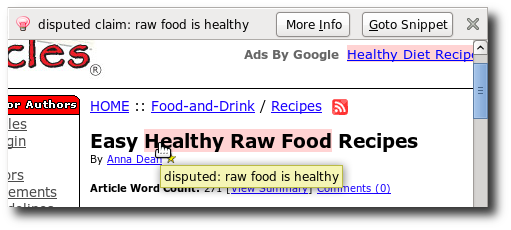
\includegraphics[width=8cm]{pictures/highlight_bar.png}
	\caption{Highlight and Notification Bar}
	\label{highlight_bar}
	\end{center}
\end{figure}

%Dispute Finder is designed to alert a user when information they read on a web page makes a claim that is disputed by a source they might trust. 
%
%
%Dispute Finder aims to inform users when information they read on the web makes claims that are disputed by sources that they might trust. We are particularly interested in informing users about claims that they hadn't thought about before, hadn't realized were disputed by sources they repect, or have not yet established a strong opinion on.

The Dispute Finder Firefox extension uses two mechanisms to inform a user when information on the page they are reading is disputed. It highlights any snippets that make the disputed claims in red, and it displays a notification bar (Figure~\ref{highlight_bar}). 

The notification bar alerts the user that they should look out for highlighted snippets. Highlights can be difficult to see if the page is using a background that is similar to our highlight color\footnote{We tried to choose a color that is easily distinguished from most background commonly used background colors} or if the user is color blind. The notification bar also allows a user to step through the highlighted snippets on the page.

The highlights show a user {\it which phrases} Dispute Finder believes are making disputed claims. This allows a user to ignore disputed claims that are made by text that the user isn't interested in - such as user comments. The highlights also allow a user to see when Dispute Finder has incorrectly inferred that a phrase as making a disputed claims that it isn't making. In such cases, the user is encouraged to help Dispute Finder improve its marking by clicking on the disputed claim and clicking on the "report incorrect highlighting" button from the popup interface.

Once a user is aware that a claim is disputed, there is little point telling them about the same disputed claim again in the future. We have not yet concluded whether it is better for Dispute Finder to automatically stop highlighting a claim once a user has viewed the claim, or whether it is better for a user to explicitly ask Dispute Finder to stop highlighting a claim. In our current implementation, a user can tell Dispute Finder to not highlight a claim again by setting the ``don't highlight this claim for me again'' checkbox in the popup interface (Figure~\ref{claimview}). Requiring a user to manually opt out of a claim requires more work from the user, but hiding already viewed claims can be confusing, since users do not normally expect viewing something to be a destructive operation. A compromise position is to highlight claims that have been seen before in a fainter color; similar to the way links are typically colored on web pages.

\todo{Try using a fainter color}

\todo{Text is wrong in the screenshot}

Dispute Finder also provides an API that can be used by other sites to determine whether their content makes disputed claims. For example, a search engine could inform a user if its results contained disputed claims, or an RSS feed reader could tell a user if a news story makes disputed claims.

\todo{Document API online}
\todo{Change the highlight color to yellow? Auto-adjust highlight color based on background color?}
\todo{Should we automatically adjust the highlight color, based on the background color of the page}
\todo{Discuss previous work on highlighting here, rather than in related work?}


\subsection{Explaining Disputed Claims}

If a user clicks on a highlighted snippet, Dispute Finder will bring up a popup interface explaining the different alternative points of view. We could have ommitted this feature and still had a useful system. Once a user sees that something is disputed, they could use an alternative service, such as a search engine, Wikipedia, Politifact or Snopes, to find further information about the claim. There are however several reasons why it makes sense for Dispute Finder to maintain information about a disputed claim:

\begin{description}
\item[Convenience:] A user may not have the patience to search for a good source of information about a claim. 
\item[Moderation:] We only want Dispute Finder to highlight a claim if we know that there is credible evidence for an alternative point of view - otherwise Dispute Finder would be annoying. By storing the evidence for alternative points of view inside Dispute Finder, it becomes easier for a moderator user to evaluate whether a claim is sufficiently disputed that it belongs in the Dispute Finder database.
\item[Filtering:] Although we have not implement this feature currently, we think it could be useful to build a model of what sources a user trusts and only highlight a disputed claim if a source that the user trusts argues against it.
\end{description}

Naturally, sources such as Wikipedia, Politifact, and Snopes are often used as sources of evidence for and against a claim --- indeed we currently import articles from Politifact and Snopes automatically.

We prototyped and tested two different ways of showing a user alternative points of view to the disputed claim they are looking at:

\begin{figure}[tb]
	\begin{center}
	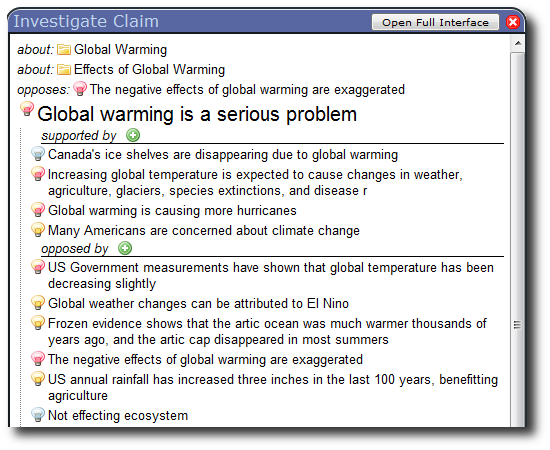
\includegraphics[width=6cm]{pictures/popup_graph_crop.png}
	\caption{Argumentation graph interface for a disputed claim}
	\label{popup_graph}
	\end{center}
\end{figure}

\begin{figure}[tb]
	\begin{center}
	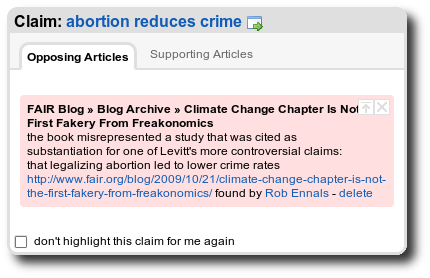
\includegraphics[width=6cm]{pictures/popup_abortion_shadow.png}
	\caption{Article List interface for a disputed claim}
	\label{article_list}
	\end{center}
\end{figure}



\begin{description}
\item[Argumentation graph:] When the user clicks on a snippet that makes a disputed claim, Dispute Finder shows them a simple user-editable argumentation graph~\cite{Conklin1987a}. Each claim is linked to claims that represent alternative points of view, and claims that support that point of view. Each claim also has a list of articles that argue in favor of that claim (Figure\ref{popup_graph})

\item[Article lists:] Dispute Finder shows the user two lists of articles, one of which contains articles arguing in favor of the claim, and the other of which contains articles arguing against the claim (Figure~\ref{article_list}). For each article, the interface shows a summary sentence that captures the core argument used by the article. A user can add any web page as a supporting article by browsing to the page, selecting "use as evidence" from a context menu (Figure~\ref{add_article}) and then saying what claim it supports or opposes (Figure~\ref{article_choose}).
\end{description}

The argumentation graph makes it easier to see {\it why} a claim is disputed, while the article lists make it easier to see {\it who} supports or opposes the claim. 

\begin{figure}[tb]
	\begin{center}
	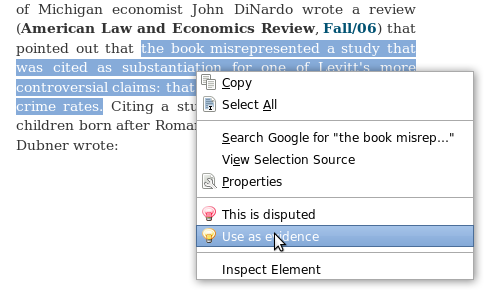
\includegraphics[width=6cm]{pictures/mark_evidence.png}
	\caption{Adding an article, with a summary sentence selected}
	\label{add_article}
	\end{center}
\end{figure}

\begin{figure}[tb]
	\begin{center}
	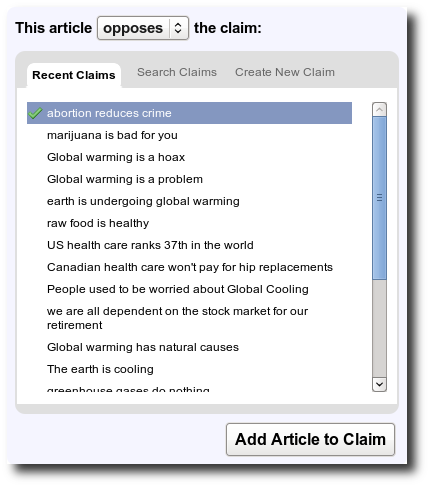
\includegraphics[width=6cm]{pictures/article_choose_claim.png}
	\caption{Choose how to connect an article with a claim}
	\label{article_choose}
	\end{center}
\end{figure}

\todo{Call them supporting pages? Naming is a mess right now.}

When using the article list approach, several different articles may be expressing essentially the same point of view and it may not be obvious that one of the articles is making a point that the user had not come across before. The argumentation graph allows the user to easily see what the range of different opinions is, and quickly see if there is an argument that they have not encountered before. 

A significant weakness of the argumentation graph approach is that a good argumentation graph takes significantly more effort to build than a simple list of articles. In our prototype the argumentation graph was built entirely by users and we found that our users had difficulty creating graphs that were useful for other users. There were two problems here: firstly, breaking down all the different arguments for and against a claim takes much more time than just adding articles to a list, particularly given that a single article will often make several different opposing points; secondly, we found that users had difficulty creating well structured argumentation graphs, as we outline in Section~\ref{user-studies}. This result is consistent with previous studies~\cite{Isenmann1997}.

Another point in favor of using a simple list of sources is that most of the users we talked to seemed to be more interested in {\it who} disputed a claim, rather than what their argument was. For example, if a user is a reader of the New York Times, and they hear that the New York Times argues against the claim they are reading, then they will take the dispute much more seriously than if the key article arguing against the claim is from a source they are not familiar with. Moreover, we found that when a user wanted to understand {\it why} a claim is disputed, they prefered to read whichever article seemed to be most credible, rather than browsing an argumentation graph.

It is possible that the best solution would be a visualisation that made it easy for a user to see both {\it who} was supporting/opposing a particular claim, and {\it why} the various sources held those opinions.


\subsection{Trustworthy Sources}

In the current version of Dispute Finder, an article can be any web page that meets the Wikipedia criteria\footnote{http://en.wikipedia.org/wiki/Wikipedia:SOURCES} for being reliable. Good sources of articles include newspapers, universities, respected organizations, and Wikipedia itself. Users can vote on whether they think a particular article is useful, and this voting determines the order in which articles are listed. A user can also request that an article be deleted if it is not relevant to the claim, or request that a claim be deleted if it is not disputed by any reliable articles. Users with moderator privileges review requests for deletion and delete claims and articles that do not meet requirements.

\todo{study result: verify}
There are significant weaknesses in this approach. Pew have shown~\cite{pew-news} that different people trust different sources. There may be little point showing liberal sources to a conservative, or vice-versa. Similarly, a global voting system can be gamed by people who vote up weak arguments against claims they support in order to hide stronger arguments. Moreover, by using moderators to decide which sources and claims are high enough quality to be presented to other users, we open ourselves up to charges of bias.

It may thus be better to learn what sources a particular user is likely to believe are reliable, and then adjust both what sources Dispute Finder shows to the user, and what claims are highlighted, based on this.

There is a difficult trade-off here. If we only show users sources that we believe they are likely to trust and only highlight claims as disputed if they are disputed by sources that share the user's own worldview then we risk reinforcing the echo-chamber effect that Dispute Finder is intended to fight against. On the other hand, if we only provide information from sources that are widely regarded as being reliable, we risk enforcing the beliefs of the establishment and stifling the voices of those who are less accepted by the establishment, but may still be right. If we pay no attention to what sources the user trusts, or what sources are regarded as respectable, then we may waste time trying to persuade users using sources that they would not take seriously. We do not yet claim to know a good solution for this problem, but we believe it is an interesting area for further research.

\todo{Cite Pew Research study saying people like to read news that supports their own point of view, but many others like neutral sources. http://people-press.org/report/?pageid=1353}


\subsection{What is Disputed?}

One of the biggest challenges in Dispute Finder, is how to build a list of disputed claims that should be highlighted for users. As discussed in Section~\ref{related:entailment}, rather than directly inferring whether a snippet is disputed by a trusted article on the web, Dispute Finder instead builds a database of known disputed claims and tries to determine whether a snippet on a web page entails the truth of one of these claims.

\todo{We are repeating information between here and the related work section on Recognizing Textual Entailment}

We do not want the database of disputed claims to contain everything that has every been disputed by anyone. In some sense almost everything is disputed by someone on the web. There are enough people writing enough opinions that if we alerted users every time anything they read was disputed by anyone then Dispute Finder would would be so distracting as to be worthless. Similarly, there is little point spending effort rebutting claims that nobody believes. For example there is reliable evidence that the moon is made of cheese, but few people believe this claim is true. What we want is a set of claims that are widely believed and for which there is credible evidence supporting other points of view.

\begin{figure}[tb]
	\begin{center}
	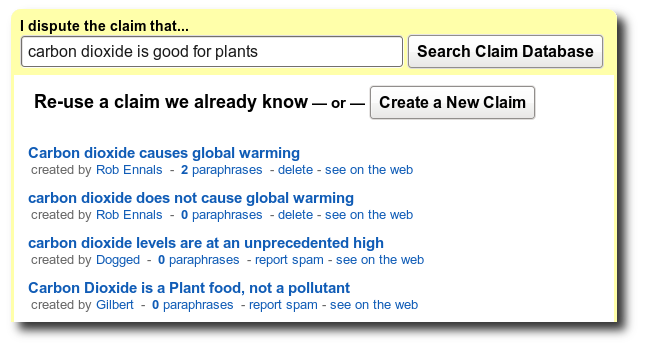
\includegraphics[width=8cm]{pictures/add_claim_list.png}
	\caption{Interface for adding a new disputed claim manually}
	\label{add_claim}
	\end{center}
\end{figure}

Fortunately, several web sites already maintain databases of disputed claims, together with arguments against them. For example Snopes.com maintains a list of urban legends and Politifact.com maintains a list of false claims about politics. We automatically import all claims that either of these sites debunk into our database and treat the sites themselves as reliable sources about the claims they debunk. In the future we intend to also import claims from other such sites, and allow users to choose which feeds of disputed claims should be used to highlight snippets on pages they browse.

We also allow users to add their own disputed claims using the Dispute Finder web interface (Figure\ref{add_claim}). The web interface is modeled after common issue-reporting software such as Uservoice.com and Bugzilla.org. It first encourages the user to search the existing database to see if their claim already exists, and then allows them to create a new claim. When the claim is first added it is marked with a warning, informing the user that the claim will not be highlighted for other users until they have added at least one opposing article.

The automatic import feeds allow Dispute Finder to bootstrap a large database of disputed claims without needing a large active user community and the crowdsourcing aspect allows users to clean up claims that were not phrased well when imported, and add claims that are not part of any of our input feeds.

\todo{Say how many disputed claims}

\todo{talk about duplicates}

\todo{Actually import the Politifact data}

\subsection{Finding Snippets}

Given a web page that the user is browsing, and a database of claims that we believe are disputed, how can we determine what snippets on the page are making claims that are in our database? We implemented and tested four approaches:

\begin{figure}[tb]
	\begin{center}
	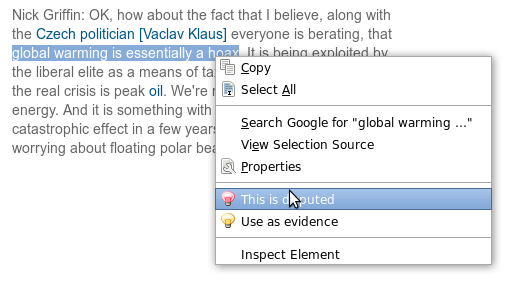
\includegraphics[width=6cm]{pictures/mark_disputed.png}
	\caption{Explicit page marking}
	\label{mark_disputed}
	\end{center}
\end{figure}

\begin{figure}[tb]
	\begin{center}
	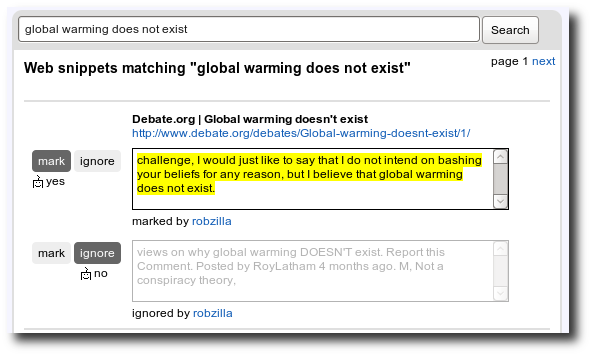
\includegraphics[width=7cm]{pictures/training.png}
	\caption{Bulk page marking}
	\label{training}
	\end{center}
\end{figure}


\begin{description}
\item[Explicit page marking:] If the page a user is reading contains a snippet that makes a disputed claim, the user can mark that snippet by selecting it, right clicking, and selecting "mark as disputed" from a popup menu.

\item[Bulk page marking:] The user enters a paraphrase of the claim into a web UI. The server searches the web for snippets that resemble this phrase using Yahoo BOSS~\cite{boss?} and shows the user the snippets it found. The user clicks on all of the snippets that they would like to mark.

\item[Server-side classification:] The server uses the examples from the bulk page marking interface to train a classifier. We used a simple baysian classifier with n-grams as its features. As the user gives examples of snippets that do or do not entail the original claim, the classifier learns what n-grams should or should not be in a snippet. Once the classifier is sufficiently trained, the server applies it to the rest of the results from Yahoo BOSS to automatically mark web pages. We have only partially implemented this approach.

\todo{Has anyone done something like this before.}
\todo{We only partially implemented this approach}

\item[Client-side entailment:] The browser extension runs a simple textual entailment algorithm over all sentences on every web page the user browse, checking to see if any sentence on the page entails any claim in the database. A user can enter additional paraphrases of a claim to help the entailment algorithm. This is the implementation used by the currently released version of Dispute Finder.
\end{description}

Explicit page marking has the highest accuracy, but the poorest coverage. Since a user is looking at the page in its entirity, they can read the snippet in context and make a good judgement about whether the snippet is indeed making the claim. However the manual effort required per page makes it difficult for this approach to scale. It can also be hard to motivate a user to mark snippets if it is unlikely that another user with the Dispute Finder extension will read exactly this page. This is the same problem that has hindered the adoption of web page annotation tools.

Bulk page marking trades off some accuracy for better coverage. When a user searches for a phrase, they can quickly find hundreds of snippets and mark them by clicking on them. Since they are reading the snippet out of context, they are more likely to mark a phrase incorrectly. 

Server side classification trades off more accuracy for more coverage. The classifier can mark more pages than a user could ever mark manually, but is inevitably less accurate than a human.

Client side entailment gets even more coverage. Since the classification algorithm is run inside the client, the client can highlight snippets on pages that the server has not examined. This is particularly important for news pages, which are frequently read only a few minutes after they have been written. Moreover, the client-side approach can highlight snippets on web pages that would not be accessible to the server, such as web-based email, and information on an intranet.

The client side entailment method uses the standard Local Lexical Matching algorithm that is a common baseline in NLP. It divides the page into sentences, strips out stopwords, does stemming, and then looks for sentences that contain the keywords contained in a paraphrase of a known claim. If the claim contains a negation word (e.g. not, never, can't) then so must the matching sentence.

\todo{Discuss how and why this is simpler than the server-side classification method}
\todo{Explain how we avoid downloading the entire database}


The client side entailment method uses a simpler algorithm than the server-side classifier. 



\todo{Should we have a version where the interface merely suggests n-grams that should be used by the classifier}
\todo{Can we present all these systems without giving detailed stats about how they compare?}
\todo{Add support for a user to enter 'anti-phrases' when a snippet is wrongly highlighted}
\todo{Add support for a user to enter a paraphrase that will match the snippet they are looking at}
\todo{Do a load more people in a final user-study round. Try to get it up to 8.}
\todo{Explain how our algorithm relates to existing NLP work - due to unusual domain}


\section{Learning from Users}

The Design of Dispute Finder has been influenced by several different kinds of input from potential users. We performed a series of "think aloud" user studies to evaluate the user interface, we circulated a survey among members of a local debate club, and we performed a series of interviews with people selected from those who completed the survey.

\subsection{Survey}

\subsection{Interviews}

\subsection{Think-Aloud User Studies}

We performed three qualitative "think aloud" user studies. The aim of these studies was to inform the iterative design of the Dispute Finder tool. The studies were not intended to validate the design of Dispute Finder as being correct. The only way we will be able to truly validate Dispute Finder is by having it be adopted by a large community of active users - something it is not yet mature enough for.

\subsubsection{Procedure}

For the first two studies, we recruited participants using Craigslist. We posted a message asking people to tell us how they used the web to form and promote their opinions, and used this to select people who we thought might fit our "skeptical reader" and "activist" personas. After these studies, we decided that the kind of person who looks for jobs of craigslist is unlikely to be a good fit for our personas, and so for the final study we instead used people we knew personally and thought fit our personas well. All study groups were small. The first study had twelve participants (five female, seven male), the second study had six participants (four female, two male), and the final study had ?? participants (?? male, ?? male). 

Each batch of users was shown a different iteration of the Dispute Finder design. The first two batches used versions in which users marked snippets explicitly, and the popup window for a claim showed an argumentation graph describing the structure of the different alternative points of view. The final group used a version in which a textual entailment algorithm on the client was used to determine what to mark, and the popup window showed lists of sources that support or oppose the claim. We present the findings of the three user studies together. Where a comment refers to particular version we make this clear.

Study sessions took approximately fourty five minutes. Participants were seated at a workstatation with the Firefox browser augemented with the Dispute Finder extension. They were asked to view pages that had highlighted claims on them, and to attempt to add new disputed claims to our database.

\todo{Need to finish the third wave of user studies}

\subsubsection{Findings}

Response was generally positive, with many participants being very keen to use the tool soon. Several participants asked as to notify them when it is properly deployed. Most of the participants expressed an interest in using the tool, with some wanting to use it now, and others wanting to use it ``when it is more mature''.

Most participants said that they would want to use Dispute Finder to tell them when information they read was disputed (skeptical reader). One participant said ``The web needs to be taken with a grain of salt, and this gives you salt goggles''. A smaller number said they would be likely to enter claims they disagreed with (activist). One participant who was a political blogger was very excited about the mark things he thought were lies.

Most users were able to use Dispute Finder compentently as a skeptical reader (browsing information about disputed claims) but found it harder to act compentently as an activist (adding new disputed claims).

When browsing a page that had disputed claims highlighted, most users correctly inferred that these were sentences they should be skeptical about, but some users thought that we were saying they were wrong, rather than merely disputed. Not all users realised that one could click on a disputed claim to bring up more information.

%In the first study, a user could mark a snippet by 
%
%In the interface used in the first two studies, a user could mark a snippet by selecting it, right clicking on it, and clicking "mark as disputed". They were then prompted to either select an existing claim or create a new one.

When asked to mark snippets on a particular page that make disputed claims, users often did not appreciate that they should either re-use existing claims or create claims that would be applicable to snippets on many other pages. Several users tried to create a new claim with exactly the same text as the snippet they were marking, and several users asked why they had to "enter the text again". Similarly, users got confused when a snippet made two different disputed claims. The correct behavior is to mark the same text with two different claims, but several participants tried to create a new compound claim such as "Global warming will cause X and Y". 

Conversely, when adding a claim to the Dispute Finder web site, users would often enter claims that are not disputed anywhere on the web, or enter paraphrases that do not resemble the wording used on any web site. The challenge of how to help users come up with claims that occur on many web sites is one that we have not yet solved.

Several users expressed confusion about how specific a claim they created should be. For example, if a snippet says ``Global temperatures will rise by X degrees by 2050'' then is that making the claim ``Global temperatures will rise'', or should the claim include the extra information? In order to make a good judgement, one needs to know the range of similar claims that are being made by other web sites, and what claims one has good evidence against. If one makes the claim too specific then one will be able to find less web pages that make it, but if one makes the claim too general then it might be harder to find solid evidence against it.

When adding sources that support or oppose a claim, a user would frequently mark the first paragraph of the article rather than seeking out the sentence that best summarized the argument that the article was using against the claim. In some cases the first paragraph is indeed the right text to select, since the first paragraph is typically a summary of the core argument made by the articles. Several users wanted to mark up a table or image as the summary of an article, which is not currently supported.

In the first two studies, the popup interface for a claim showed an argumentation graph. This graph connected the graphs in our database using "supports" or "opposes" links, and allowed each claim to also be associated with supporting articles. 

When shown an argumentation graph for a claim, users seemed to have little difficulty navigating and understanding it and appreciated the ability to explore the structure of an argument and see how different claims were connected. One user said "I can see myself getting addicted to this", and another said "it's very intuitivet".

Users seemed to have difficulty creating such graph structures however. Some users linked one claim as supporting another when it would have been more logically correct for them to both support a third claim. For example "Global warming is causing more hurricanes" does not support "Global warming is causing rising sea levels", but both support "Global warming is causing problems". Users correctly realised that the claims were related, but were not sure how best to connect them. Some users were confused by claims that had a ``because'' relationship rather than a ``supports'' or ``opposes'' relationship. For example ``America did not sign the Kyoto Protocol'' {\it because} ``Signing Kyoto would harm the US economy''. It is possible that creating logically correct claim structures may be too difficult for some people (see Isenmann and Reuter~\cite{Isenmann1997}).

Several users got confused by claims that referred to similar events at different points in time. For example, one participant in the first study marked one claim as opposing another claim when they were referring to similar incidents that occurred at different times. 

When using the article-list interface, several users got confused about whether an article supported or opposed a claim that was itself phrased in the negative. For example a user would mark an article that opposed global warming as opposing the claim "global warming is bad" because the article opposed global warming.

Several users expressed an interest in being able to add a disputed claim without having to find opposing evidence. One user said that opposing a claim required ``too many clicks'' and they wanted to be able to just vote against a claim without having to say why or find evidence. 

Several users created claims that had ambiguous meanings. One user entered a disputed claim about "Wood", meaning the guitarist "Ronnie Wood" of the Rolling Stones. Similar problems occured with claims that were specific to a particular country, or a particular point in time. 

The biggest problem that Dispute Finder has right now is that it is rare that Dispute Finder will highlight a snippet that makes a claim that the user did not already know was disputed. This is for two reasons: our database of disputed claims is currently too small (around two thousand claims at the time of writing), and our textual entailment algorithm is not sufficiently sophisticated to stand a good chance of highlighting snippets when they make those claims.

\todo{Need to say that the argumentation graph contains all existing claims and that it was a simple "supports"/"oppsose" graph.}.

\todo{Come up with terminology for marking an evidence snippet, and agree on evidence vs source vs article}
\todo{Talk about how the early versions conflated evidence and snippets - and whether it makes sense to distinguish between them}
\todo{Screenshot of the claim graph interface}


\section{Conclusions and Future Work}

We have introduced the idea of creating an Open Hypermedia system that automatically highlight snippets on the web that are disputed by sources you might trust. We have explored several different design options, tested multiple variants on users, and reported insights from this testing.

An experimental preview version of Dispute Finder is available at the following URL:
\url{http://disputefinder.org}

Performing these tasks well is a hard problem, and we do not yet claim to have an implementation that is is good enough to be compelling for most users. We do however believe that Dispute Finder attacks an interseting problem that, if solved well, could significantly improve the utility of the web.


\section{Acknowledgments}

\todo{Do we want to have acknowledgements}
% We would like to Thank Barbara Rosario for help with textual entailment, and 
% Acknowledgements omitted for blind submission. Dispute Finder uses icons from the free FamFamFam Silk\footnote{http://famfamfam.com} collection.


\todo{Sort out bad references}
\bibliography{refs}

\end{document}



